\chapter{Optimization and Resampling Algorithms} \label{chp:optimization}
\epigraph{Great quote.}{Author}
\begin{figure}[H]
	\centering
	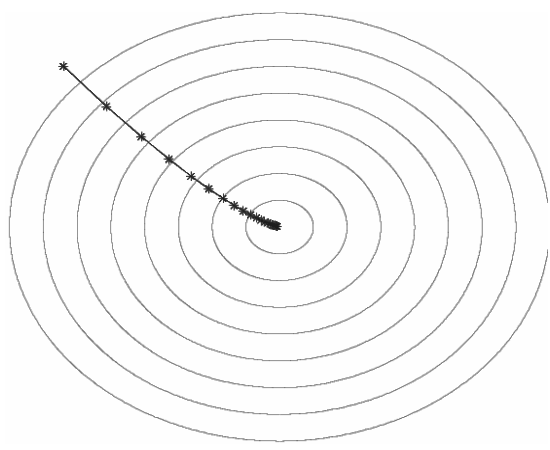
\includegraphics[scale=0.5]{Images/gd_bw.png}
	\caption{An iterative optimization algorithm is always approaching an extremum in a possibly multi-dimensional space. Here illustrated in a two-dimensional space where the equipotential curves are drawn.}
\end{figure}

In this chapter, we will cover the remaining algorithms we need before we can move on to the implementation. A good optimization algorithm is a must, we need an algorithm which can treat a large number of parameters because of the restricted Boltzmann machines. For that reason, we will introduce the ADAM optimizer, which has gained an extreme popularity after is was presented in 2014.  We also need an algorithm 

\newpage
\section{Optimization algorithms}
In chapter \ref{chp:machinelearning}, we discussed the gradient descent optimization algorithm, which is among the most basic methods available. That method is based on the gradient, which is the slope of the cost function, but many methods are also in need of the Hessian matrix, which gives the curvature of the cost function. We will overlineely scratch the surface of this field, limiting us to the gradient methods. 

To have the method fresh in mind, we will start with reintroducing the gradient descent method before we move on the its stochastic brother. We will then have a look at how momentum can be added, and finally we examine the stochastic and momentum based ADAM optimizer. 

\subsection{Gradient descent} \label{sec:gd}
Perhaps the simplest and most intuitive method for finding the minimum is the gradient descent method, which reads
\begin{empheq}[box={\mybluebox[5pt]}]{align}
\label{eq:GD}
\bs{\theta}_t=\bs{\theta}_{t-1} - \eta\nabla_{\theta} \mathcal{C}(\bs{\theta}_{t-1})
\end{empheq}
where $\bs{\theta}_t$ is the parameter vector at time step (iteration) $t$ and $\eta$ is the learning rate. $\nabla_{\theta} \mathcal{C}(\bs{\theta}_{t-1})$ is the gradient of the cost function with respect to all the parameters $\theta$ at time $t-1$. 

The idea is to find the direction where the cost function $\mathcal{C}(\bs{\theta})$ has the steepest slope, and move in the direction which minimizes the cost function. For every time step, the cost function is thus minimized, and when the gradient approaches zero the minimum is found. A possible, but basic, stop criterion is
\begin{equation}
\nabla_{\theta} \mathcal{C}(\bs{\theta}_t)<\varepsilon.
\end{equation}
where $\varepsilon$ is a tolerance. More robust methods are based on comparing the value of the cost function for several past iterations. 

In cases where the cost function is not strictly decreasing, we will have both local and global minima. Often, it is hard to say whether we are stuck in a local or global minimum, and this is where the stochasticity enters the game.

\subsection{Stochastic gradient descent}\label{sec:sgd}
Stochastic gradient descent is closely related to the gradient descent method, but the method uses randomly selected batches to evaluate the gradients, hence the stochasticity. By introducing this randomness, the parameters will not always be updated in order to minimize the energy, which makes us less likely to be stuck in a local minimum.

In practice, one splits the data set in $n$ batches, and select one of them to be used in the parameter update. Our hope is that this batch is representative for the entire data set, such that the new parameters gives a lower cost function. If that is the case, we have reduced the cost of an iteration significantly, since we only need to care about a batch. After each batch in the data set has had an opportunity to update the internal parameters, we say that we have went through an \textit{epoch}.

We are not guaranteed that updating the parameters with respect to a batch gives a lower cost function, and when it is not, we need to run more batches in order to minimize the cost function. Since each iteration is faster than for standard gradient descent, this is acceptable. As long as the batch is slightly representative for the entire data set, the cost function will be minimized in the end.

Mathematically, the method can be expressed as 
\begin{empheq}[box={\mybluebox[5pt]}]{align}
\label{eq:SGD}
\bs{\theta}_t=\bs{\theta}_{t-1} - \eta\nabla_{\theta} \mathcal{C}_i(\bs{\theta}_{t-1})
\end{empheq}
where we use the $i$'th batch in the parameter update. Standard gradient descent is actually just a special case of this, where we only have one batch ($i$ includes the whole data set). If we still get stuck in local minima after adding the stochasticity, it might be a good idea to add momentum as well.

\subsection{Adding momentum} \label{sec:momentum}
If we go back to an introductory mechanics course, you might remember that momentum is a quantity that maintains the motion of a body. Imagine a ball that rolls down a steep hill, but then there is a local minimum that it needs to escape to keep rolling. If it has enough momentum, it will be able to escape.

Exactly the same idea lies behind the momentum used in optimization algorithms; the momentum will try to maintain the motion towards the global minimum, which makes the system less likely to be stuck in a local minimum.  

Momentum can be added to most optimization algorithms, also gradient descent and stochastic gradient descent. The way we do it is to save the direction we were moving in the previous iteration, and use it as a contribution to the next gradient update. A typical implementation of the first-order momentum looks like
\begin{empheq}[box={\mybluebox[5pt]}]{equation}
\begin{aligned}
\bs{m}_t &= \gamma\bs{m}_{t-1} + \eta\nabla_{\theta} \mathcal{C}_i(\bs{\theta}_{t-1})\\
\bs{\theta}_t&=\bs{\theta}_{t-1}-\bs{m}_t
\end{aligned}
\end{empheq}
where $\gamma$ is the momentum parameter, which is just another hyper-parameter usually initialized to a small number. $\bs{m}_t$ is the momentum vector, and can be initialized as the zero vector.

The optimization algorithm can be modified further in unlimited ways. A common improvement is to add higher order momentum, another is to make the learning rate adaptive. We have implemented the most basic version of this, with monotonic adaptivity. Many algorithms, such as the conjugate gradient method, also make use of the Hessian as discussed in the introduction, but that is another level of complexity. 

We will end this section with setting up the algorithm of a stochastic gradient descent optimization with momentum and monotonic adaptivity. The algorithm is found in algorithm \eqref{alg:asgd}.

\begin{algorithm}
	\SetAlgoLined
	\Parameter{$\eta$: Learning rate}
	\Parameter{$\gamma$: Momentum parameter}
	\Parameter{$\lambda$: Monotonic decay rate}
	\Require{$\mathcal{C}(\bs{\theta})$: Cost function}
	\Data{$\bs{\theta}_0$: Initial parameters}
	
	$\bs{m}_0\leftarrow 0$ (Initialize momentum vector)\;
	$t\leftarrow 0$ (Initialize time step)\;
	\While{$\bs{\theta}_t$ not converged}{
		$t\leftarrow t+1$ (Increase time for each iteration)\;
		$\bs{g}_t\leftarrow \nabla_{\theta}\mathcal{C}_t(\bs{\theta}_{t-1})$ (Get gradients from a given batch at time $t$)\;
		$\bs{m}_t\leftarrow \gamma\bs{m}_{t-1}+\eta\cdot\bs{g}_t$ (Update first momentum estimate)\;
		$\bs{\theta}_t=\bs{\theta}_{t-1}-\eta\cdot\bs{m}_t/\lambda^t$ (Update parameters)\;
	}
	\KwResult{Updated parameters $\bs{\theta}_t$ after convergence}
	\caption{Adaptive stochastic gradient descent with momentum. See sections (\ref{sec:sgd}-\ref{sec:momentum}) for details. Robust default settings for the hyper-parameters are $\eta=0.001$, $\gamma=0.01$ and $\lambda=0.1$. All the operations are element-wise.}
	\label{alg:asgd}
\end{algorithm}

\subsection{ADAM}
ADAM is a first-order stochastic optimization method which is widely used in machine learning. It was discovered by D.P. Kingma and J. Ba, and published in a 2014 paper. The article has already more than 25000 citations! \cite{kingma_adam:_2014} So what makes this method so popular? 

The main reason why it is widely used, is obviously that it performs good. The fact that it only requires the gradient makes it efficient, and the way the momentum is implemented still makes able to handle a large number of parameters. 

The optimization algorithm can be expressed as a set of equations
\begin{empheq}[box={\mybluebox[5pt]}]{equation}
\begin{aligned}
\bs{g}_t&=\nabla_{\theta} \mathcal{C}_t(\bs{\theta}_{t-1})\\
\bs{m}_t&=\gamma_1\bs{m}_{t-1}+(1-\gamma_1)\bs{g}_t\\
\bs{v}_t&=\gamma_2\bs{v}_{t-1}+(1-\gamma_2)\bs{g}_t^2\\
\hat{\bs{m}}_t&=\bs{m}_t/(1-\gamma_1^t)\\
\hat{\bs{v}}_t&=\bs{v}_t/(1-\gamma_2^t)\\
\bs{\theta}_t&=\bs{\theta}_{t-1}-\eta\hat{\bs{m}}_t/(\sqrt{\hat{\bs{v}}_t}+\bs{\varepsilon})
\end{aligned}
\end{empheq}
where $\bs{m}_t$ is the biased first momentum estimate of the parameter vector $\bs{\theta}$ and $\bs{v}_t$ is the biased second raw moment estimate. The momentum parameters need to be in the range $\gamma_1,\gamma_2\in[0,1)$, and are often set to values close to 1. This makes the optimization adaptive: as time goes, the factors $1-\gamma_1^t$ and $1-\gamma_2^t$ approach 1 from below. $\eta$ corresponds to the learning rate, and should be a small number. Finally, the parameter $\varepsilon$ is added to avoid division by zero. 

We can set up the algorithm in a similar manner to the adaptive stochastic gradient descent algorithm from above, which gives the algorithm \eqref{alg:adam}.

\begin{algorithm}
	\SetAlgoLined
	\Parameter{$\eta$: Learning rate}
	\Parameter{$\gamma_1,\gamma_2\in [0,1)$: Momentum parameters}
	\Parameter{$\varepsilon$: Division parameter}
	\Require{$\mathcal{C}(\bs{\theta})$: Cost function}
	\Data{$\bs{\theta}_0$: Initial parameters}
	
	$\bs{m}_0\leftarrow 0$ (Initialize 1$^{\text{st}}$ momentum vector)\;
	$\bs{v}_0\leftarrow 0$ (Initialize 2$^{\text{st}}$ momentum vector)\;
	$t\leftarrow 0$ (Initialize time step)\;
	\While{$\bs{\theta}_t$ not converged}{
		$t\leftarrow t+1$ (Increase time for each iteration)\;
		$\bs{g}_t\leftarrow \nabla_{\theta}\mathcal{C}_t(\bs{\theta}_{t-1})$ (Get gradients from a given batch at time $t$)\;
		$\bs{m}_t\leftarrow \gamma_1\bs{m}_{t-1}+(1-\gamma_1)\cdot\bs{g}_t$ (Update first momentum estimate)\;
		$\bs{v}_t\leftarrow \gamma_2\bs{v}_{t-1}+(1-\gamma_2)\cdot\bs{g}_t^2$ (Update second raw momentum estimate)\;
		$\hat{\bs{m}}_t\leftarrow\bs{m}_t/(1-\gamma_1^t)$ (Bias-corrected first momentum estimate)\;
		$\hat{\bs{v}}_t\leftarrow\bs{v}_t/(1-\gamma_2^t)$ (Bias-corrected second momentum estimate) \;
		$\bs{\theta}_t\leftarrow\bs{\theta}_{t-1}-\eta\cdot\hat{\bs{m}}_t/(\sqrt{\hat{\bs{v}}_t}+\bs{\varepsilon})$ (Update parameters) \;
	}
	\KwResult{Updated parameters $\bs{\theta}_t$ after convergence}
	\caption{ADAM optimizer. Robust default settings for the hyper-parameters are $\eta=0.001$, $\gamma=0.01$ and $\lambda=0.1$. All the operations are element-wise, and for in-depth information see the original paper, \cite{kingma_adam:_2014}.}
	\label{alg:adam}
\end{algorithm}

\section{Variance estimation}
In experiments, we have two main classes of errors, systematical errors and statistical errors. The former is a result of external factors such as uncertainties in the apparatus or a person constantly takes an incorrect measurement, which an error that is hard to estimate. The latter, however, can be found by estimating the variance and we are therefore interested in finding an accurate variance at a low cost. Monte-Carlo simulations can be treated as computer experiments, and therefore we can use the same analyzing tools as we do for real experiments. 

There are several ways to estimate the variance, where the cheapest ones also are the less accurate ones. To make the most use of our data, we use resampling methods to estimate the statistical errors. Some well-known resampling algorithms are blocking, bootstrap and jackknife. We will cover the blocking method only, since that is the only one we use in our particular implementations. To save computational time, we resample the final iteration only, for the others we use the simple estimation method.

Before we go through the methods, we will give a brief introduction to some useful statistical quantities. We start with the \textit{moments}, which are given by
\begin{equation*}
\langle x^n\rangle=\int dxx^np(x)
\end{equation*}
where $p(x)$ is the true \textit{probability density function}. If we know this function, we had not have to estimate the statistical errors, but as it is unavailable in real experiments, the moments can only be estimated. The first moment is the \textit{mean} of $p$, and is often denoted by the letter $\mu$
\begin{equation}
\langle x\rangle=\mu=\int dxxp(x)\approx \frac{1}{n}\sum_{i=1}^n x_i=\overline{x}_n.
\end{equation}
Furthermore, we can define the \textit{central moments}, which are given by
\begin{equation}
\langle(x-\langle x\rangle)^n\rangle=\int dx(x-\langle x\rangle)^2p(x)
\end{equation}
which is centered around the mean. With $n=0$ and $n=1$, this is easy to find, but what is the central moment with $n=2$? The central moment with $n=2$ is what we call the variance, and is often denoted as $\sigma^2$ as we did in the equation \eqref{eq:variance}. One can show that
\begin{equation}
\sigma^2=\langle(x-\langle x\rangle)^2\rangle=\langle x^2\rangle - \langle x \rangle^2
\label{eq:variance2}
\end{equation}
which was already stated in the theory chapter. For a sampling, the corresponding quantity can be found from
\begin{equation}
\sigma^2=\frac{1}{n-1}\sum_{i=1}^n(x_i-\langle x\rangle)^2\approx \frac{1}{n-1}\sum_{i=1}^n(x_i-\overline{x})^2
\end{equation}
which is very cheap to compute. However, as an estimate of the sample variance, this is poor if the ...
This is very cheap to compute as we only need the mean of the local energy squared, $\overline{E_L^2}$, but as a sample variance of a data set $X$, $V(\overline{X})$ it is a poor estimate since it does not account for the covariance between the measurements. This covariance is essential when the measurements are correlated, and leads to equation \eqref{eq:variance2} being an underestimation of $V(\overline{X})$, and is thus more a guideline for the size of the uncertainty, more than an actual estimate of it. For a stationary time series $X$ consisting of $n$ subsets $X_i$, the variance can be written as
\begin{equation}
\begin{aligned}
V(\overline{X})&=V\bigg[\frac{1}{n}\sum_{i=1}^nX_i\bigg]=\frac{1}{n^2}\text{Cov}\bigg[\sum_{i=1}^nX_i,\sum_{j=1}^nX_j\bigg]\\
&=\frac{\sigma^2}{n}+\frac{2}{n}\sum_{h=1}^{n-1}\Big(1-\frac{h}{n}\Big)\gamma(h)
\end{aligned}
\label{eq:samplevariance}
\end{equation}
where $\gamma(h)$ is the autocovariance function which describes the covariance of a set of time points in a series with another set of time points in the same series. The covariance gives the correlation between two set of data $X_i$ and $X_j$ according to
\begin{equation}
\text{Cov}(X_i,X_j)=\langle(X_i-\langle X_i\rangle)(X_j-\langle X_j\rangle)\rangle\approx \langle(X_i-\overline{X})(X_j-\overline{X})\rangle,
\end{equation}


Fortunately, there are computational methods that can
calculate $\sigma^2$ with the covariance contribution included. The method used in
this project is the blocking method, which follows.

\subsection{Blocking}\label{sec:resampling}
Above, we have described the need of a proper estimation of the uncertainty in computational simulations, where the covariance was included in
the calculation of $\sigma^2$. A quick and easy way to get a proper estimate of the uncertainty, is by using the blocking method.

When the blocking method was made popular by Flyvberg and Peterson in 1989, the method required hyper-parameters which had to be carefully adjusted for each particular data set. \cite{flyvbjerg_error_1989} In 2018, Marius Jonsson reinvented the algorithm and made it automated, with no need for external parameters. Despite this, no compromise was made on performance. The method scales as $12n+\mathcal{O}(\log_2n)$ for small data sets, but reduces to $n+\mathcal{O}(1)$ for large data sets, which makes it preferred over bootstrap and jackknife for large data sets. \cite{jonsson_standard_2018} We will now go through the idea behind the blocking method.

Consider a time series $\{x_1, x_2, \hdots, x_n\}$ with $n=2^d$ data point for some integer $d>1$. For this case, an autocovariance function $\gamma(h)$ is guaranteed to exist. We arrange the data in a vector
\begin{equation}
X=(x_i,x_2,\hdots,x_n),
\end{equation}
which we assume to be asymptotically uncorrelated. The idea is to take the mean of subsequent pair of elements from $X$, and form a new vector $X_1$. We then repeat the operation on $X_1$ and form a new vector $X_2$ and so on. This is the reason why we require $n=2^d$. If $k$ denotes an element in vector $X_i$, we can write the procedure recursively as
\begin{equation}
\begin{aligned}
(X_0)_k&\equiv(X)_k\\
(X_{i+1})_k&\equiv\frac{1}{2}\Big((X_i)_{2k-1}+(X_i)_{2k}\Big)
\end{aligned}
\end{equation}
where $1\leq i\leq d-1$ and $1\leq k\leq n/2^i$. According to equation \eqref{eq:samplevariance}, we have that
\begin{equation}
V(\overline{X}_k)=\frac{\sigma_k^2}{n_k}+\frac{2}{n_k}\sum_{h=1}^{n_k-1}\Big(1-\frac{h}{n_k}\Big)\gamma_k(h)
\end{equation}
Where we define the last term as the \textit{truncation error}, $e_k$, as it is intractable. It can be shown that the sample variance of all pairs $(X_i)_k$ and $(X_j)_k$ after a while will be identical \cite{flyvbjerg_error_1989},
\begin{equation}
V(\overline{X}_i)=V(\overline{X}_j)
\label{eq:varivarj}
\end{equation}
with the consequence that
\begin{equation}
V(\overline{X})=\frac{\sigma_k^2}{n_k}+e_k\quad\text{for all}\quad 0\leq k\leq d-1.
\end{equation}
In the original (manual) blocking method, we had to know exactly where to stop the procedure in order to equation \eqref{eq:varivarj} to hold. If we do not continue long enough, the sample variance has not converged, while if we keep on going for too long, the standard error of $V(\hat{\sigma}_k^2/n_k)$ get very large. If one plots the sample variance as a function of the iterations, one will see that the curve forms a plateau before it gets very noisy, but with Jonsson's automated method, we do not need to worry about this. 

We will end this section by scratching the most basic blocking algorithm

\IncMargin{1em}
\begin{algorithm}
	\SetAlgoLined
	\Parameter{$\eta$: Learning rate}
	\Parameter{$\gamma$: Momentum parameter}
	\Parameter{$\lambda$: Monotonic decay rate}
	\Require{$\mathcal{C}(\bs{\theta})$: Cost function}
	\Data{$\bs{\theta}_0$: Initial parameters}
	
	$\bs{m}_0\leftarrow 0$ (Initialize momentum vector)\;
	$t\leftarrow 0$ (Initialize time step)\;
	\While{$\bs{\theta}_t$ not converged}{
		$t\leftarrow t+1$ (Increase time for each iteration)\;
		$\bs{g}_t\leftarrow \nabla_{\theta}\mathcal{C}_t(\bs{\theta}_{t-1})$ (Get gradients from a given batch at time $t$)\;
		$\bs{m}_t\leftarrow \gamma\bs{m}_{t-1}+\eta\cdot\bs{g}_t$ (Update first momentum estimate)\;
		$\bs{\theta}_t=\bs{\theta}_{t-1}-\eta\cdot\bs{m}_t/\lambda^t$ (Update parameters)\;
	}
	\KwResult{Updated parameters $\bs{\theta}_t$ after convergence}
	\caption{Adaptive stochastic gradient descent with momentum. See sections (\ref{sec:sgd}-\ref{sec:momentum}) for details. Robust default settings for the hyper-parameters are $\eta=0.001$, $\gamma=0.01$ and $\lambda=0.1$. All the operations are element-wise.}
	\label{alg:asgd}
\end{algorithm}\DecMargin{1em}

In our work, we will consequently use Marius Jonsson's automated blocking algorithm and code, available on \url{https://github.com/computative/block}.

\section{Summary of the algorithms}
Up to this point we have presented several algorithms, and to give the reader a complete description of the simulating procedure, we will here summarize them and place them in the correct order. First, Metropolis-Hastings algorithm was given, which is responsible for the sampling. Thereafter, we presented a few optimization algorithms, before we gave the blocking algorithm. 

The optimization loop forms the outer environment

\IncMargin{1em}
\begin{algorithm}
	\SetAlgoLined
	
	\Parameter{$\eta$: Learning rate}
	\Parameter{$\Delta x$: Step length}
	\Require{$\Psi_T(\bs{r},\bs{\theta})$: Trial wave function}
	\BlankLine
	$\bs{r}\leftarrow \mathcal{N}(0,\sigma^2)$ (Initialize positions randomly)\;
	$\bs{r}\leftarrow \mathcal{U}(0,1)$ (Initialize parameters, could be randomly)\;
	\While{not converged}{ 
		$E_L=[-]$ (Declare an empty local energy list)\;
		$grad=[-]$ (Declare an empty parameter gradient list)\;
		$ELgrad=[-]$ (Declare an empty list containing parameter gradient $\cdot$ local energy)\;
		\For{$i\leftarrow 1$ \KwTo $M$}{
			$\bs{r}\leftarrow\bs{r}+\Delta x$ (Update position)\;
			\If{$\Psi_T(\bs{r}_{\text{new}})/\Psi_T(\bs{r}_{\text{old}})<\mathcal{U}(0,1)$}{
				reject move \;
			}
			$E_L^i\leftarrow \big(\hat{\mathcal{H}}\Psi_T(\bs{r},\bs{\theta})\big)/\Psi_T(\bs{r},\bs{\theta})$ (Fill $E_L$-list with local energies) \;
			$grad^i\leftarrow \nabla_{\theta}\ln\Psi_T(\bs{r})$ (Fill grad-list with parameter gradients) \;
			$ELgrad^i\leftarrow E_L^i\cdot grad^i$ (Fill ELgrad-list) \;
		}
	}
	\KwResult{Updated parameters $\bs{\theta}_t$ after convergence}
	\caption{Adaptive stochastic gradient descent with momentum. See sections (\ref{sec:sgd}-\ref{sec:momentum}) for details. Robust default settings for the hyper-parameters are $\eta=0.001$, $\gamma=0.01$ and $\lambda=0.1$. All the operations are element-wise.}
	\label{alg:asgd}
\end{algorithm} \DecMargin{1em}







